\chapter{Introduction}

\textcolor{blue}{(6-10 pages) This chapter should contain: Motivation. Context e.g. a R\&D project. Problem definition. 
Research questions. Summary of main results/contributions. Clarification of possible contributions from co-authors. 
Outline of rest of thesis. We suggest the following subchapters:}

\section{Problem Outline}
\textcolor{blue}{Motivate the thesis, why is your topic an interesting one?}

\section{Research Context}
\textcolor{blue}{In what context have you been working? Was it an externally financed project, did that put restrictions or directions on your research directions?}

\section{Research Questions}
\textcolor{blue}{Name your research questions, outline briefly why these are interesting. Do not go too in depth here, remember it is only an introductory chapter they will be covered more thorough in later chapters.}

\textcolor{blue}{RQ1:\ldots}

\textcolor{blue}{RQN:\ldots}

\section{Research Design}
\textcolor{blue}{Outline how your research has been happening, figures, timelines and tables that connect papers, 
research questions and studies are a nice help here to create an overview of the work - see Figure
\ref{fig:1-studies_contributions_papers}.}


\begin{figure}
\begin{center}
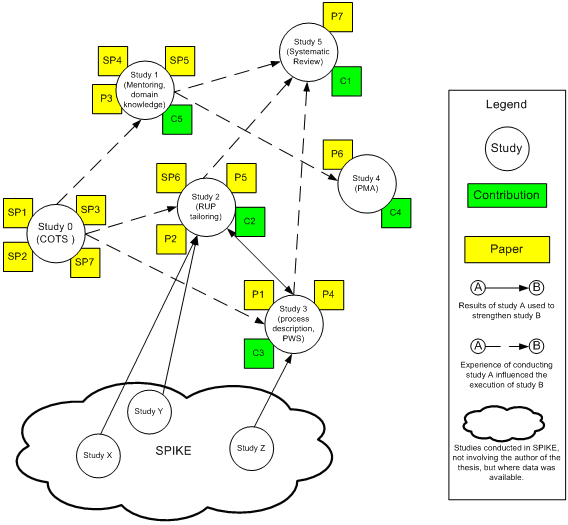
\includegraphics[width=.75\textwidth]{../img/1-studies_contributions_papers} \caption[Example studies vs. contributions 
vs. papers]{Example studies vs. contributions vs. papers [Bj{\o}rnson�s PhD thesis]}
\label{fig:1-studies_contributions_papers} 
\end{center}
\end{figure}


\section{Papers}
\textcolor{blue}{If your thesis is an article thesis, provide a list of your included papers here with full 
bibliography. If you want to go more in depth here you could include abstracts, identify their relevance to the thesis 
and your contributions towards them. Keep in mind you are still in the introduction chapter and you should keep it as 
short as possible.}


\begin{table}[!h]
\begin{tabular}{lp{.8\textwidth}} 

\textcolor{green}{P1} &

\textcolor{green}{Finn Olav Bj�rnson and Tor St�lhane: "Harvesting Knowledge through a Method Framework in an Electronic 
Process Guide", Proc. 7th International Workshop on Learning Software Organizations (LSO), Kaiserslautern, Germany, 
2005, 107-111 (Post conference proceedings printed in Springer LNAI 3782, 2005, 86-90)}

\textcolor{green}{\textbf{Relevance to this thesis:} This paper presents our initial findings in study 3, and details 
how they envisioned their knowledge sharing project. It describes a tool based on the preferences of the developers and 
input from the research literature. The paper answers research question RQ2.1 and contributes towards contribution C3 
and to some degree C2. The study contributes to a small degree towards research theme RT2.}

\textcolor{green}{\textbf{My contribution:} This paper is the result of a cooperation in SPIKE. I performed half of the 
interviews during the data gathering and was responsible for performing the analysis of the qualitative data. I was the 
leading author of this paper.} \\

\end{tabular}
\end{table}

	

\section{Contributions}
\textcolor{blue}{Identify and list your contributions in the thesis, provide a short description of each contribution.}

\textcolor{blue}{C1: \ldots}

\textcolor{blue}{C2: \ldots}

\textcolor{blue}{+++}


\begin{table}[!h]
\centering
\begin{tabular}{|l|l|l|l|l|} 
\hline
\textcolor{green}{Research} & \textcolor{red}{Question} & \textcolor{red}{Contribution} & \textcolor{red}{Papers} & \textcolor{red}{Focus} \\
\hline
\textcolor{red}{RQ1} & \textcolor{red}{C1}, \textcolor{red}{C2} & \textcolor{red}{P4} & \textcolor{red}{P7} & \textcolor{red}{COTS} \\
\hline

\end{tabular}
\caption{Example of relations}
\label{tab:1-relations}
\end{table}


\section{Thesis Structure}
\textcolor{blue}{Briefly outline the rest of your thesis:}

Chapter 2: State of the Art

Chapter 3: Context and Research Design

Chapter 4: Results

Chapter 5: Evaluation and Discussion of Results

Chapter 6: Conclusion

Appendix A: (enclosed, selected papers)

Appendix B: (basic info incl. abstracts of secondary papers)

\ldots

Appendix N: lab results and other data, empirical tools like questionnaires, enclosures. 



\section{Examples REMOVEME!}

This is an example of a reference \cite{copland2000}.

This is a reference to Table \ref{tab:1-relations} and to Figure \ref{fig:1-studies_contributions_papers}.

A glossary example which will be included in the glossary at the end of the document:
% \glossary{name=Newton,description=Unit of force but may also refer to Sir Isaac Newton.}

An abbrevation example which will be included in the list of abbrevations: 
%\abbr{name=NTNU,description=Norwegian University of Science and Technology}

% To use the glossary:
% 1. Compile the latex document.
% 2. Run the makeGlossary.{bat|sh} (.bat for windows, .sh for Linux/Unix). This script ASSUMES that your latex file is
% called document.tex 
% 3. Compile the latex document again (I have sometimes experienced some error messages but as long as I compile a
% couple of times it is ok)
